In diesem Kapitel werden die Ergebnisse der Benchmark Proben ausgewertet und die Ergebnisse aus der \texttt{pass@1} und \texttt{pass@5} Methode diskutiert. Weiterhin werden die Resultate in Bezug auf die Auswahl der Landessprache und die Wahl der Parameteranzahl bei den Modellen erläutert. Abschließend wird darauf eingegangen, wie sich die Auswahl eines Frameworks für die Interaktion mit den Modellen auf die Ergebnisse auswirken.\vspace{0.2cm}

%\sout{Diese Tests fordern LLM's auf kleine Problem zu lösen. Aus diesem Grund werden weitere Tests erstellt mit umfangreicheren Anforderungen aus dem Bereich der Webentwicklung. Zu jedem Problem wird eine Musterlösung und ein Unittest erstellt. Der Aufbau für diese Bereitstellung orientiert sich an dem Format aus dem HunamEval-Benchmark.}\vspace{0.2cm}
%Ein Versuch größere und komplexere Probleme zu lösen, hatte nicht den erwarteten Erfolg gebracht. Es sind viele Iterationen notwendig, um ein funktionierendes Ergebnis zu erhalten. Im Laufe der Iterationen sind die Prompts für die Modelle immer größer geworden und haben viele Missverständnisse bei den Modellen erzeugt. So das eine Zerlegung in kleine Probleme sich als sinnvoller erwies.\vspace{0.2cm}
%Des Weiteren ist die Bewertung der Coding-Standards der jeweiligen Programmiersprache vorgesehen. Für die Prüfung der Standards wird ein SonarQube-Server verwendet, der sowohl PHP als JavaScript unterstützt. Ebenfalls wird die Qualität des Codes evaluiert. Das Augenmerk liegt auf die Lesbarkeit, Effizienz und Wartbarkeit des generierten Codes.\vspace{0.2cm}
%Optional werden einige Tests von zusätzlichen Tools validiert, beispielsweise bei der Validierung von PHP Files sind es Tools wie phpunit\footnote{phpunit steht unter \href{https://github.com/sebastianbergmann/phpunit}{https://github.com/sebastianbergmann/phpunit} zum Download bereit.} und Code\_Sniffer\footnote{Code\_Sniffer steht unter \href{https://github.com/squizlabs/PHP_CodeSniffer}{https://github.com/squizlabs/PHP\_CodeSniffer} zum Download zur Verfügung.} für die Validierung von JavaScript findet das Framework Jasmin\footnote{\href{https://jasmine.github.io/}{https://jasmine.github.io}.} Anwendung.\vspace{0.2cm}
%---------------------------------------------------------------------------------------------------


\section{Modellbewertung}
Für die Bewertung wird das Vorgehen gewählt, welches in \cite{chen-2021} und \cite{peng-2024} beschrieben wird. Die Tests werden exemplarisch, mit der für die Webentwicklung relevanten Sprache PHP durchgeführt und in deutscher Landessprache.\vspace{0.2cm}

Aus den Ergebnissen der Tests, wird mithilfe der $pass@k$-Methode, die Zuverlässigkeit der jeweiligen Modelle berechnet. Dieser Wert gibt an, mit welcher Wahrscheinlichkeit mindestens eine richtige Lösung unter $k$ ausgewählten Vorschlägen vorhanden ist.\vspace{0.2cm}

Nachdem die fünf Versuche pro Probe ausgewertet wurden, sind die Ergebnisse in Tabelle \ref{tab:prompt_results_open_models} aufgeführt. Hier wird auf den Werten für $k=1$ und $k=5$ eingegangen. In der Tabelle sind alle getesteten Modelle nach Namen sortiert und es wird dadurch noch keine Wertung abgegeben.\vspace{0.2cm}

\begin{table}[!ht]
	\begin{tabular}{|l|r|r|}
		\hline
		\textbf{Model} & \textbf{pass@1} & \textbf{pass@5} \\
		\hline
		ChatGPT 4 API (T600)        &  0,335 &   0,6125 \\
		Codellama:13b               &  0,005 &    0,025 \\
		Codellama:70b               & 0,3325 &   0,6375 \\
		DeepSeek-Coder-V2           &  0,555 &     0,65 \\
		DeepSeek-R1                 & 0,7025 &   0,8375 \\
		Gemini Flash 1.5 Chatbot    & 0,2925 &     0,55 \\
		Gemini Flash 1.5 API (T600) &   0,06 &    0,075 \\
		Llama3.1:8b (T600)          &   0,43 &   0,6375 \\
		Llama3.1:8b (T1200)         &  0,445 &   0,6375 \\
		Llama3.1-claude:8b          & 0,4625 &     0,65 \\
		Llama3.2:3b                 & 0,2625 &     0,55 \\
		Llama3.3:70b                & 0,6275 &    0,725 \\
		Mistral-small 22b           &   0,22 &      0,4 \\
		Qwen 2.5-Coder 32b          & 0,1975 &      0,3 \\
		\hline
		\hline
	\end{tabular}
	\centering
	\label{tab:prompt_results_open_models}
	\caption{Ergebnisse der pass@1 und pass@5 Methode}
\end{table}

Die ersten Tests zur Generierung von Code wurden mit den Cloused-Source-Modellen \textit{ChatGPT 4} und \textit{Gemini 1.5} durchgeführt. Hierbei wurden die Tests mit 600 Token bei beiden Modellen durchgeführt. Insbesondere \textit{Gemini 1.5} hat mit dieser Tokenlänge Probleme. Die kurze Tokenlänge führte dazu, das die Antworten mitten in der Beantwortung der Frage unterbrochen worden. Somit waren die generierten Codefragmente nicht nutzbar. Es wurde kein lauffähiger Code generiert. Das Listing \ref{lst:humaneval_xl_prompt_23} zeigt einen unvollständig generiertes Codefragment für die Probe \textit{PHP/23}. Die Zeile sechzehn ist die letzte Zeile, welche vom Modell zurückgesandt wurde und ist zudem unvollständig.\vspace{0.2cm}

\begin{figure}[!ht]
\begin{lstlisting}[
	language=php,
	label=lst:humaneval_xl_prompt_23,
	caption={Wortlaut der Aufgabe 23 aus dem HumalEval-XL Benchmark}
]
/**
 * Sie sind ein erfahrener PHP-Programmierer und hier ist Ihre Aufgabe.
 * Gib den größten Primfaktor von n zurück. Gehe davon aus, dass n > 1 und keine Primzahl ist.
 * >>> largest_prime_factor(13195)
 * 29
 * >>> largest_prime_factor(2048)
 * 2
 *
 */
function largestPrimeFactor($n){
    $largestFactor = 1;

    // Teile n wiederholt durch 2, bis es ungerade ist
    while ($n % 2 == 0) {
        $largestFactor = 2;
        $n
\end{lstlisting}
\end{figure}

Hier wurde durch \textit{Gemini} oft zuerst die Frage wiederholt, bevor die neu generierten Teile kommen und somit die definierte Anzahl der Token nicht ausreicht, was zu einem Nachteil für dieses Modell wurde. Die gleichen Fragen wurden anschließend an den ChatBot \textit{Gemini 1.5} gestellt, was zu einem besseren Ergebnis führte. Während die Gemini API mit 600 Token für den \texttt{pass@1} einen Wert von 6\% erreichte waren es bei den Abfragen des Gemini ChatBots 29,3\%.\vspace{0.2cm}

Das Modell \textit{ChatCPT 4} von OpenAI wurde über die API abgefragt. Hierbei lag der Wert für den \texttt{pass@1} bei 33,5\% und der Wert für den \texttt{pass@5} bei 61,25\%. Weitere Tests wurden aufgrund der Kosten mit diesem Modell nicht weitergeführt. Somit ist die Ermittlung der Werte für die \texttt{pass@k} Methode bei einer höheren Tokenlänge nicht mehr erfolgt.\vspace{0.2cm}

Eines der getesteten Open-Source-Modelle ist das \texttt{codellama} Modell mit 13 Milliarden Parametern. Dieses hat beim Generierung der PHP Lösungen aus dem Proben des Benchmarks am schlechtesten abgeschnitten. Der Grund hierfür war, dass die meisten generierten Codes für die Programmiersprache Python erstellt worden. Das ist der Grund warum die meisten Tests, welche durch den Benchmark vorgegeben waren, ein negatives Ergebnis auswiesen. Das zweite der Codellama-Familie ist das Modell mit 70 Milliarden Parametern. Dieses Modell erreichte beim \texttt{pass@1} ein Ergebnis von 33,25\% und erreicht mit ChatGPT identische Werte. Während dieses Modell bei der Evaluation des \texttt{pass@5} den gleichen Wert 63.75\%, wie das Llama3.1 erreicht und somit über dem Ergebnis von ChatGPT 4 liegt.\vspace{0.2cm}

Des Weiteren wurden eine Reihe von Llama-Modellen getestet, darunter verschiedene Llama3.1 Modelle. Bei dem \textit{Llama3.1 8b} wurden zwei verschiedene Versuche durchgeführt mit jeweils unterschiedlicher Tokenlängen. Anders als bei dem Modell \textit{Gemini 1.5 (API)} können die kleineren Modelle schon mit geringerer Tokenlänge valide Antworten erzeugen. Die unterschiedliche Tockenlängen haben kaum einen Einfluss auf das Ergebnis. Hier wies das Llama 3.1 mit 1200 Token gegenüber dem Llama 3.1 mit 600 Token eine Verbesserung von 1,5\% bei der \texttt{pass@1} Methode auf. Bei der Auswertung der \texttt{pass@5} Werte, war keine Veränderung der Ergebnisse zu beobachten, hier liegt der Wert konstant bei 63,75\%.\vspace{0.2cm}

Um einen Ansatz zur Optimierung der Prompts zu testen, wurde das Modell \textit{Llama3.1-Claude 8b-q4} ebenfalls evaluiert. Bei diesem Modell handelt es sich um ein \textit{Llama 3.1:8b} Model, welches mit den System Prompts des Modells \textit{Claude Sonnet 3.5} von der Firma Anthroppic erstellt wurde. Bei der Lösungsgenerierung wurden die Antworten beide Modelle mit 600 Token limitiert. Hier konnte eine Verbesserung gegenüber dem Basismodell um 3,25\% für den \textit{pass@1} und um 1,25\% für den \textit{pass@5} festgestellt werden. Die Ergebnisse sind in Tabelle \ref{tab:prompt_results_open_models} und in der Abbildung \ref{img:pass_at_k_results_by_llm} zu sehen.\vspace{0.2cm}

\begin{figure}[!ht]
	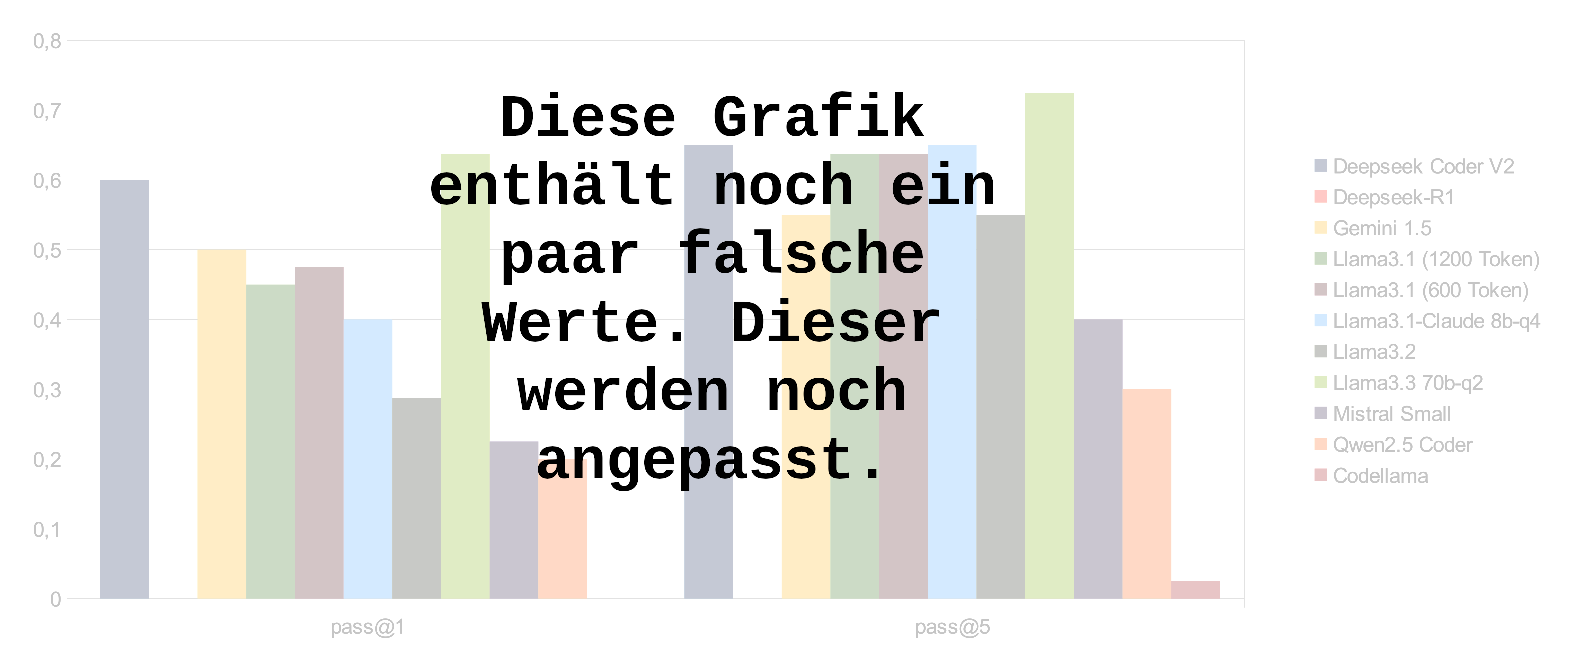
\includegraphics[width=\textwidth]{content/chapter_evaluation/images/llm_evaluation.eps}
	\centering
	\caption{Ergebnisse der pass@k-Methode für die Modelle}
	\label{img:pass_at_k_results_by_llm}
\end{figure}

Ein weiteres getestetes Modell aus dem Hause \textit{Meta} ist das Modell \textit{LLama3.2:3b}. Es ist mit 3 Milliarden Parameter kleiner als das getestete Vorgängermodell \textit{Llama3.1:8b} und somit das kleinste welches in dieser Arbeit evaluiert wird. Diesem Modell erzielte bei der Generierung von PHP Code, beim \texttt{pass@1} eine Wahrscheinlichkeit von 26,25\% und beim \texttt{pass@5} eine Wahrscheinlichkeit von 55\%.\vspace{0.2cm}

Ein letztes Modell aus der Llama3 Reihe, das dem Benchmark unterzogen wurde, ist das \textit{Llama3.3 70b-instruct-q2\_K}. Mit einem pass@1 Ergebnis von 62,75\% und 72,5\% beim pass@5 liefert dieses Modell das drittbeste Ergebnis. Bei dem vorliegenden Modell handelt es sich um ein quantisiertes Modell, was die Größe des Modells auf rund 26 GB reduziert. Bei diesem Modell wurde einige Komponenten einer 2-Bit Quantisierung unterzogen und eine fast gleichbleibende Ausgabenqualität liefern. Weitere Informationen zu diesem Modell sind \cite{hugging-face-2025} zu entnehmen. Das Basismodell mit ca. 43 GB ließ sich nicht mit den verfügbaren lokalen Ressourcen testen.\vspace{0.2cm}

Ebenfalls wurden zwei Open-Source-Modelle von der KI-Entwicklungsfirma Deepseek evaluiert.
Das Modell \textit{Deepseek Coder V2 16b} erreichte bei der Auswertung des \texttt{pass@1} eine Wahrscheinlichkeit von 55,5\% und beim \texttt{pass@5} eine Wahrscheinlichkeit von 65\%. Somit liegt es in der Bewertung des Benchmarks für den \texttt{pass@1} mit 12,5\% vor den \textit{Llama3.1} und mit 29,25\% vor dem \textit{Llama3.2} Modell und ist somit erzielte das Modell deutlich bessere Werte. Beim \texttt{pass@5} liegt das Modell mit dem \textit{Llama31-Claude}, mit 65\% gleich. Identische Werte lieferte auch die Evaluation mit der \texttt{pass@5} Methode im Vergleich zu den \textit{Llama3.x} Modellen. Das \textit{Deepseek Coder V2} Modell lag von dem \textit{Llama3.1}, mit 1,25\% und vor dem \textit{Llama3.2}, mit 10\%. Ähnliches ergab die Auswertung der \texttt{pass@5} Methode. Hier lag \textit{Deepseek Coder V2} 7,5\% hinter dem \textit{LLama3.3} Modell.\vspace{0.2cm}

Das zweite Modell von der KI-Entwicklungsfirma DeepSeek, welches evaluiert wurde, ist das Modell \textit{DeepSeek-R1}. Dieses Modell hat die besten Ergebnisse erzielt, obwohl es mit 32 Milliarden Parameter nicht das größte von den getesteten Modellen ist, erreicht es bei der Evaluierung der \texttt{pass@1} Methode 70,25\% und beim \texttt{pass@5} 83,75\%. Somit liegt es beim \texttt{pass@1} 7,5\% vor dem \textit{Llama 3.3} und bei der Auswertung des \texttt{pass@5} sind es 11,5\% vor dem \textit{Llama3.3} Modell.\vspace{0.2cm}

Zusätzlich wurden zwei weitere Modelle aus dem Open-Source-Bereich in die Evaluation einbezogen: \textit{Mistral-Small:22b}, entwickelt von der KI-Entwicklungsfirma MistralAI, sowie \textit{Qwen2.5 Coder:32b} von Qwen-AI. \textit{Mistral  Small} hat bei er Evaluation des \texttt{pass@1} ein Ergebnis von 22\% und beim \texttt{pass@5} ein Ergebnis von 40\%. Das Modell \texttt{Qwen2.5 Coder} erreicht beim \texttt{pass@1} ein Ergebnis von 19,75\% und beim \texttt{pass@5} ein Ergebnis von 30\%. Somit ist die Wahrscheinlichkeit eine korrekte Antwort unter den TOP Antworten zu generieren etwa nur halb so groß wie bei den getesteten \textit{Llama3.1} Modellen.


\subsection{Evaluierung der Parametergröße}
Eine weitere Untersuchung soll zeigen, ob es einen Zusammenhang gibt, zwischen der Modellparameteranzahl und der \textit{Wahrscheinlichkeit das sich eine korrekte Antwort unter $k$ Probe befindet}. Somit soll die Evaluation aufzeigen, inwieweit die Anzahl der Parameter die Ausgaben beeinflusst und ob die Auswahl eher auf große Modelle fallen sollte. Die Abbildung \ref{img:results_by_llm_param} zeigt die getesteten Modelle, in Abhängigkeit ihre Parametergröße und ihren Ergebnissen bei der \texttt{pass@1} Methode für die deutsche Sprache. Die Größeneinheit für die Parameterangaben ist in Milliarden und die Angaben der \texttt{pass@k} Methode in Prozent. In dieser Arbeit werden nur die Open-Sorce-Modelle verglichen, da keine offiziellen Daten zu den Parametern der Cloused-Source-Modelle bereitgestellt werden.\vspace{0.2cm}

\begin{figure}[!ht]
	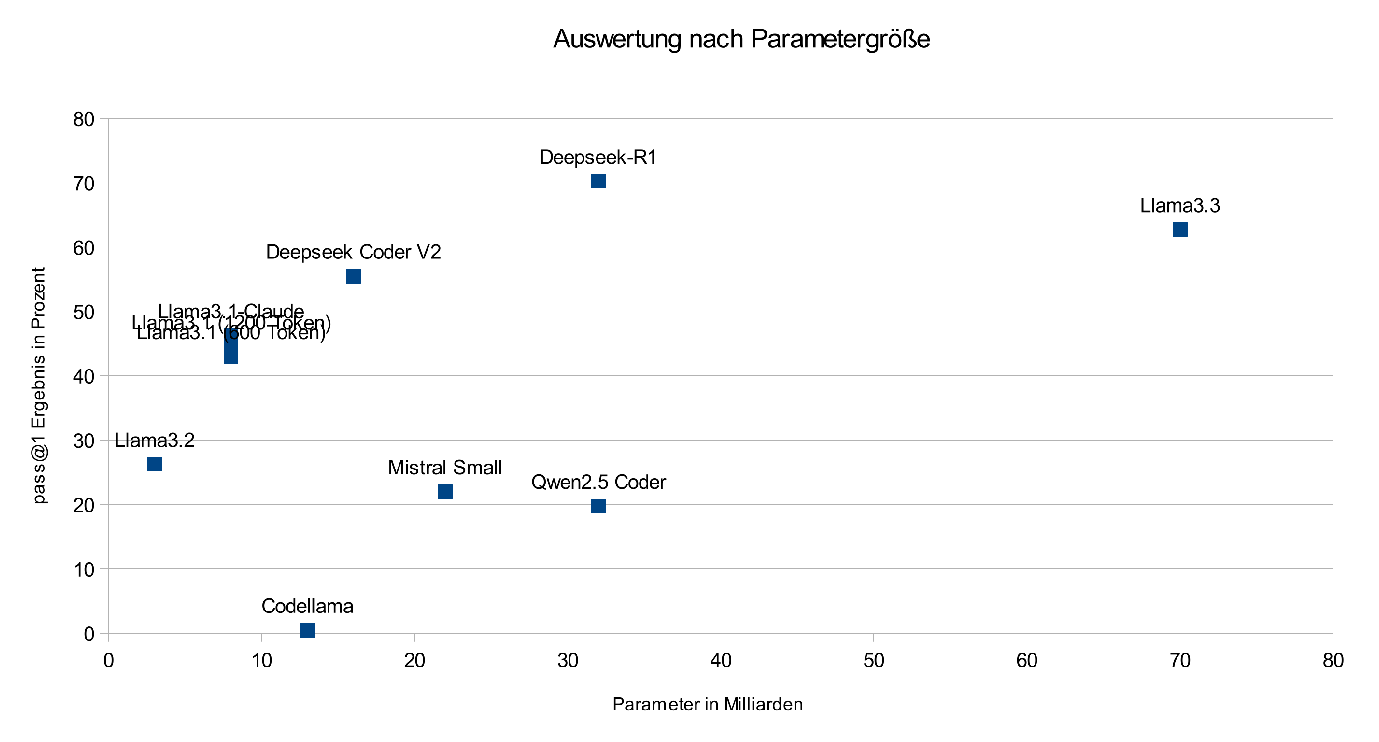
\includegraphics[width=\textwidth]{content/chapter_evaluation/images/llm_evaluation_param.eps}
	\centering
	\caption{Ergebnisse der pass@k-Methode für die Modelle}
	\label{img:results_by_llm_param}
\end{figure}

Die hier getesteten Modelle sind eher kleine Modelle und lassen sich in drei Gruppen aufteilen. Die erste Gruppe sind Modelle mit weniger oder genau \textit{10b} Parametern, in der zweiten Gruppe werden alle Modelle die großer \textit{10b} sind und bis \textit{32b} reichen und schließlich die dritte Gruppe umfasst alle Modelle die größer als \textit{32b} sind.\vspace{0.2cm}

% 1. Gruppe
Die kleineren \textit{Llama3.1:8b} Modelle übertreffen in der Evaluierung die Modelle der zweiten Gruppe \textit{Mistral Small:22b}, \textit{Qwen2.5 Coder:32b} und \textit{Codellama:13b}. Die \textit{Llama3.1:8b} Modelle liegen in ihrer Gruppe deutlich über dem \textit{Llama3.2:3b} Modell.\vspace{0.2cm}

% 2. Gruppe
Bei den Modellen zwischen 11b und 32b haben die Modelle von Deepseep \textit{Coder V2} und \textit{R1} die besten Ergebnisse. Das \textit{Deepseek-R1} übertrifft sogar die größten hier getesteten Modelle \textit{Llama3.3:70b} und \textit{Codellama:70b}. Während die Modelle \textit{Mistral Small} und \textit{Qwen2.5-Coder} deutlich unter den Ergebnissen der Deepseek-Modelle liegen.\vspace{0.2cm}

% 3. Gruppe
Bei den Modellen mit 70 Milliarden Parameter liegt das \textit{Llama3.3} vor dem \textit{Codellama} Modell. Jedoch liegen beiden getesteten Modelle unter den Ergebnissen des \textit{Deepseek-R1} Modell, welches nur 32 Milliarden Parameter aufweist. Das \textit{Deepseek Coder V2} Modell mit 13 Milliarden Parametern und die \textit{LLama3.1} Modelle mit 8 Milliarden Parametern, erzielten ebenfalls besser Ergebnisse als das \textit{Codellama} Modell.\vspace{0.2cm}

% Ergebnis
Somit lässt sich feststellen, dass bei den hier getesteten Modellen kein Zusammenhang zwischen der Anzahl der Parameter und der Qualität des generierten Codes besteht und die Anzahl der Parameter nicht ausschlaggebend ist, um eine gute Codequalität zu gewährleisten.\vspace{0.2cm}

Die Ergebnisse aus diesem Test sind in Tabelle \ref{tab:prompt_results_open_models_by_param} zusammengefasst und zeigen die genauen Werte, für die Ergebnisse des Benchmarks, welche in der Abbildung \ref{img:results_by_llm_param} grafisch dargestellt sind.

\begin{table}[!ht]
	\begin{tabular}{|l|r|r|}
		\hline
		\textbf{Model} & \textbf{Parameter} & \textbf{pass@1} \\
		\hline
		Codellama:13b         & 13 &  0,005 \\
		Codellama:70b         & 13 & 0,3325 \\
		Qwen2.5 Coder         & 32 & 0,1975 \\
		Mistral Small         & 22 &   0,22 \\
		Llama3.2              &  3 & 0,2625 \\
		Llama3.1 (600 Token)  &  8 &   0,43 \\
		Llama3.1 (1200 Token) &  8 &  0,445 \\
		Llama3.1-Claude       &  8 & 0,4625 \\
		Deepseek Coder V2     & 16 &  0,555 \\
		Llama3.3              & 70 & 0,6275 \\
		Deepseek-R1           & 32 & 0,7025 \\
		\hline
		\hline
	\end{tabular}
	\centering
	\label{tab:prompt_results_open_models_by_param}
	\caption{Ergebnisse der pass@1 Methode mit Angabe der Parameter}
\end{table}


\subsection{Evaluierung nach Sprache}
Eine Überprüfung, inwieweit die englische Sprache besser Ergebnisse liefern würde, wurde exemplarisch mit den \textit{Llama}-Modellen \textit{3.1:8b}, \textit{3.2:3b} und \textit{3.3:70b} durchgeführt. Alle drei Modelle repräsentieren unterschiedliche Anzahl der Parameter und somit verschiedene Modellgrößen.\vspace{0.2cm}

Ein Grund für diese Annahme ist, die in Kapitel \ref{subsec:disadvantages_of_evaluation} gezeigten Fehler, die bei der Übersetzung der Proben festzustellen war.
Es kann auch nicht ausgeschlossen werden, dass die Trainingsdaten für die Modelle Fehler in der Übersetzung enthalten. Diese könnten ebenfalls zu falsch generiertem Code, in einer nicht englischen Sprache führen. Aus den genannten Gründen, lag die Vermutung nahe, dass eine Evaluierung in der englischen Sprache, wesentlich bessere Ergebnisse liefern könnte. Diese Vermutung wurde auch durch die Auswertungen in \cite[][11]{peng-2024} (Tabelle 12), bei denen die Programmiersprache PHP, in der englischen Version im Durchschnitt besser abschnitt bestärkt.\vspace{0.2cm}

Diese Vermutung konnte mit den durchgeführten Tests der ausgewählten Modelle nur bedingt bestätigt werden. Das \textit{Llama3.3} zeigt beim pass@1, in der englische Version einen besseren Wert. Hier betrug der Unterschied 3,5\%, bei denen die Ergebnisse in Deutsch einen Wert von 62,75\% erreichten. Die Werte nähert sich mit steigendem $k$ Wert an, sodass bei $k=5$ die Ergebnisse in Englisch und Deutsch identisch sind und beide Sprachen einen Wert für die Wahrscheinlichkeit von 72,5\% erreichten.\vspace{0.2cm}

Das \textit{Llama3.2} Modelle zeigte beim \texttt{pass@k} für $k=1,...,5$ ein umgekehrtes Verhalten, als das zuvor genannte \textit{Llama3.3} Modell. Mit einem steigendem $k$-Wert erzielte diese Modellvariante immer bessere Resultate in der deutschen Sprache. Für den \texttt{pass@1} erzielte das \textit{Llama3.2} Modell für die deutschen Proben einen Wert von 26,25\% und bei den englischen Proben einen Wert von 24,75\%. Einen Wert von 45\% konnte für das englische Modell beim \texttt{pass@5} festgestellt werden und das deutsche Modelle erreichte einen Wert von 55\%. Somit betrug der Unterschied bei den Ergebnissen des Benchmarks, beim \texttt{pass@1} gerade einmal 1,5\%, während es beim \texttt{pass@5} bereits 10\% waren.\vspace{0.2cm}

Ein ausgeglichenes Resultat zeigt das \textit{Llama3.1} Modell, bei dem Vergleich beider Sprachen. Hier sind die \texttt{pass@3} Resultate in Deutsch und Englisch fast identisch und der Unterschied liegt hier bei 0,75\%. Während bei abnehmenden $k$-Werten die englischen Resultate besser werden, ist bei zunehmenden $k$-Wert eine Verbesserung der deutschsprachigen Ergebnisse zu erkennen. Für den \texttt{pass@1} ist das englische Ergebnis von 48,5\% um 5,5\% besser als die Resultate mit dem deutschen Proben des Benchmarks. Beim \texttt{pass@5} lagen die Ergebnisse in Deutsch, mit 63,75\% um 2,5\% vor den englischen Ergebnissen.\vspace{0.2cm}

In der Abbildung \ref{img:pass_at_k_results_by_llama_lang} werden die Ergebnisse der $pass@k$-Methode mit $k=1 … 5$ für die ausgewählten Llama-Modelle zusammengefasst. Die Proben wurden jeweils in Englisch und in Deutsch an die Modelle gestellt.\vspace{0.2cm}

\begin{figure}[!ht]
	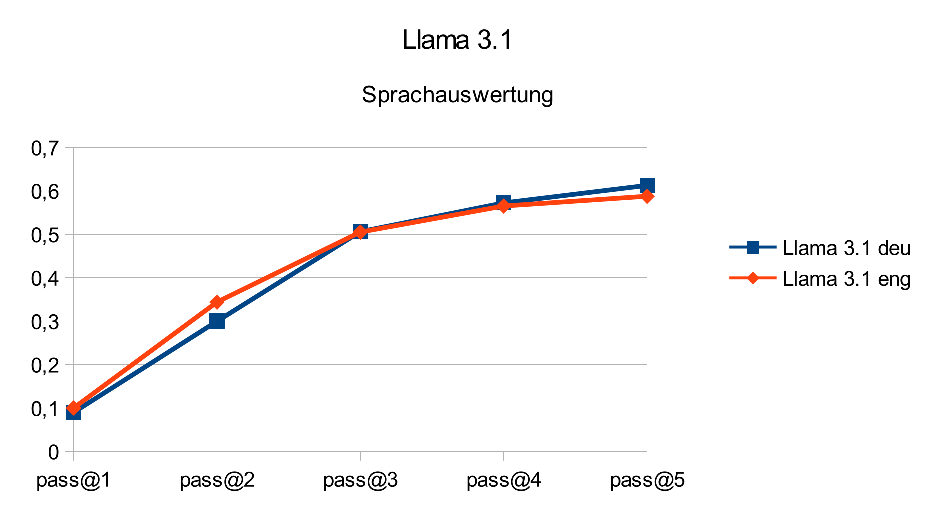
\includegraphics[width=0.45\textwidth]{content/chapter_evaluation/images/llama31_evaluation_lang.eps}
	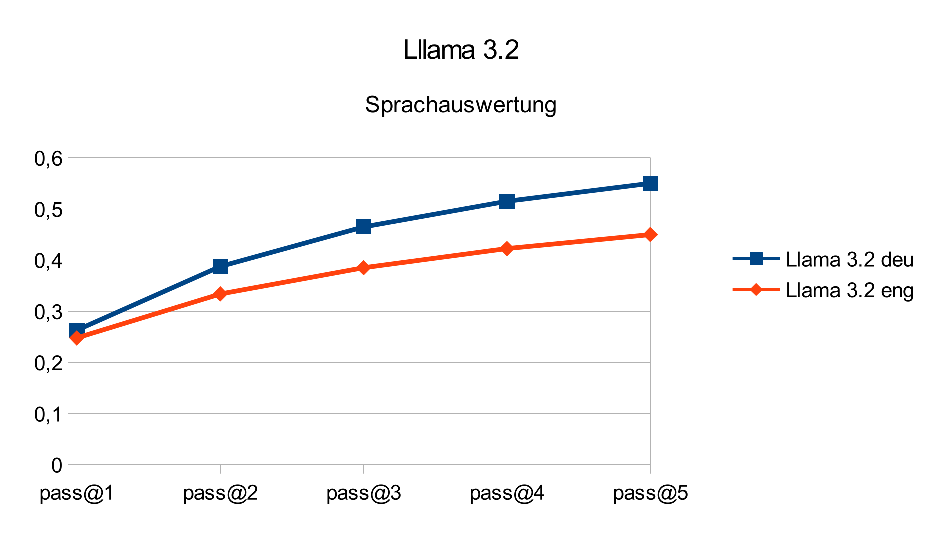
\includegraphics[width=0.45\textwidth]{content/chapter_evaluation/images/llama32_evaluation_lang.eps}
	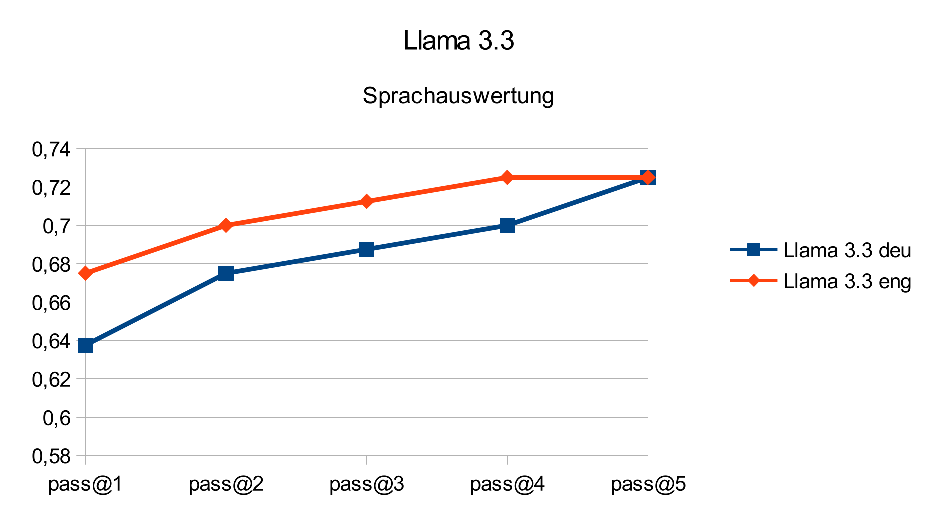
\includegraphics[width=0.45\textwidth]{content/chapter_evaluation/images/llama33_evaluation_lang.eps}
	\caption{Ergebnisse der pass@k-Methode für Llama Modelle in gewählten Sprachen}
	\label{img:pass_at_k_results_by_llama_lang}
\end{figure}

Die Tabelle \ref{tab:prompt_results_llama_x_by_lang} dokumentiert die Resultate des Benchmarks für die \textit{Llama3.x} Modelle. Hier sind alle Werte für die \texttt{pass@k}, mit $k=1,...,5$ notiert. Die Differenz zwischen der deutschen und englischen Sprachen wurde nach der Formel $DE - ENG = diff$ berechnet. Somit stellt eine positive Differenz, ein besseres Ergebnis für die Proben in Deutsch dar und eine negative Differenz ein besseres Ergebnis für die Proben in Englisch dar.\vspace{0.2cm}

\begin{table}[!ht]
	\begin{tabular}{|l|lll|lll|lll|}
		\hline
		& \multicolumn{3}{c|}{\textbf{Llama3.1}} & \multicolumn{3}{c|}{\textbf{Llama3.2}} & \multicolumn{3}{c|}{\textbf{Llama3.3}} \\
		%\hline
		\textbf{k} & \textbf{DE} & \textbf{ENG} & \textbf{diff} & \textbf{DE} & \textbf{ENG} & \textbf{diff} & \textbf{DE} & \textbf{ENG} & \textbf{diff} \\
		\hline
		1 & 0,43 & 0,485 & -0,055     & 0,2625 & 0,2475 & 0,015  & 0,6275 & 0,6625 & -0,035 \\
		2 & 0,5375 & 0,5512 & -0,0137 & 0,3875 & 0,3337 & 0,0538 & 0,6825 & 0,6987 & -0,0162 \\
		3 & 0,59 & 0,5825 & -0,0075   & 0,465 & 0,385 & 0,08     & 0,7063 & 0,7125 & -0,0062 \\
		4 & 0,62 & 0,6 & 0,02         & 0,515 & 0,4225 & 0,0925  & 0,7175 & 0,72 & -0,0025 \\
		5 & 0,6375 & 0,6125 & 0,025   & 0,55 & 0,45 & 0,1        & 0,725 & 0,725 & 0 \\
		\hline
		\hline
	\end{tabular}
	\centering
	\label{tab:prompt_results_llama_x_by_lang}
	\caption{Vergleich der englischen und deutschen Sprache für den \texttt{pass@1}}
\end{table}

Dieser Test zeigt, dass eine deutschsprachige Verwendung der Modelle nicht zwangsläufig schlechteren Code generiert.

%--- Optimierung -----------------------------------------------------------------------------------


\section{Optimierung der Ergebnisse durch die Wahl des Frameworks}
% https://ki-techlab.de/ki-news/evaluierung-grosser-sprachmodelle-ein-technischer-leitfaden/
Um zu prüfen, ob sich mit verschiedenen Frameworks Optimierungen erzielen lassen, wurden die Modelle \textit{Codellama}, \textit{Llama3.1}, \textit{Mistral Small} und \textit{Qwen 2.5 Coder} herangezogen. Von den vier getesteten Modellen zeigten drei eine signifikante Verbesserung in den Ergebnissen. Nur das im Test verwendetet Llama3.1 Modell hat nach der Änderung des Frameworks eine Verschlechterung der Ergebnisse gezeigt. Bei diesem Modell sank das Ergebnis beim \texttt{pass@1} um 0,095 von 0,43 auf 0,335 und beim \texttt{pass@5} sank das Ergebnis des Tests von 0,6375 auf 0,6125\%.\vspace{0.2cm}

Bei den getesteten Modellen \textit{Codellama} und \textit{Mistral Small} wurde eine erhebliche Verbesserung festgestellt. Beim \textit{Codellama} Modell erhöhte sich das Ergebnis des Benchmarks beim \texttt{pass@1} um 0,1425 von 0,005 auf 0,1475 und beim \texttt{pass@5} um 0,375 von 0,025 auf 0,4. Eine ähnliche Verbesserung zeigt das Modell \textit{Mistral Small}. Hier stiegt der Wert des Ergebnisses beim \texttt{pass@1} um 0,3175 von 0,22 auf 0,5375 und beim \texttt{pass@5} um 0,325 von 0,4 auf 0,725.\vspace{0.2cm}

Die besten Werte, nach der Framework Änderung erzielte das Modell \textit{Qwen 2.5 Coder}. Hier ist ein Anstiegt der Ergebnisse beim \texttt{pass@1} um 0,515 und beim \texttt{pass@5} um 0,525 zu beobachten. Somit erreicht das Modell im Benchmark für den \texttt{pass@1} ein Ergebnis von 0,7125 und für den \texttt{pass@5} einen Wert von 0,825. Mit diesem Ergebnis liegt das \textit{Qwen 2.5 Coder} Modell fast gleich auf mit dem neusten Modell von Deepseek, dem \textit{Deepseek-R1} Modell. Dieses hat im Benchmark, mit dem \texttt{langchain} Framework einen Wert für den \texttt{pass@1} von 0,7025 und für den \texttt{pass@5} von 0,8375 erreicht.\vspace{0.2cm}

Die Ergebnisse des Vergleichs der beiden Frameworks \texttt{langchain} und \texttt{DSPy} werden in den Diagrammen der Abbildung \ref{img:pass_at_k_results_by_framework} dargestellt. Jedes Diagramm zeigt die Ergebnisse eines Modells für den \texttt{pass@1} und für den \texttt{pass@5} mit beiden Frameworks.\vspace{0.2cm}

\begin{figure}[!ht]
	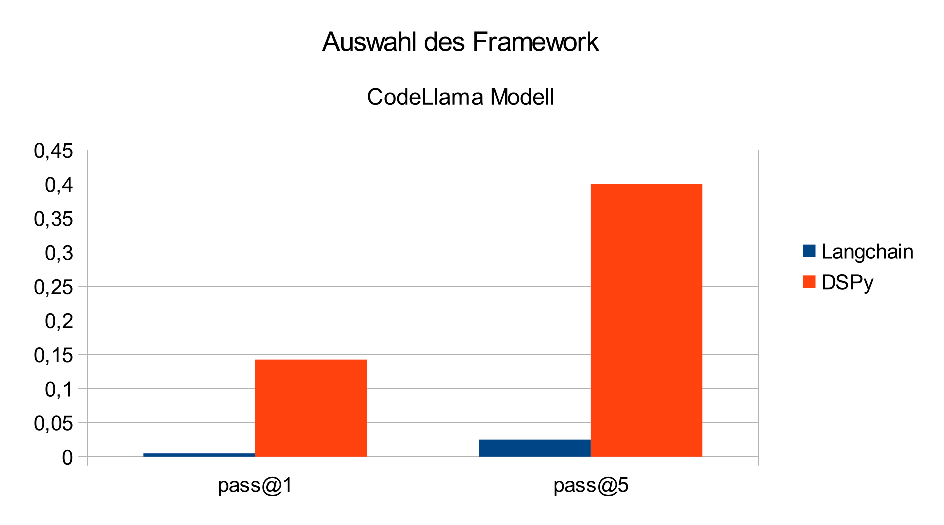
\includegraphics[width=0.5\textwidth]{content/chapter_evaluation/images/framework_evaluation_codellama.eps}
	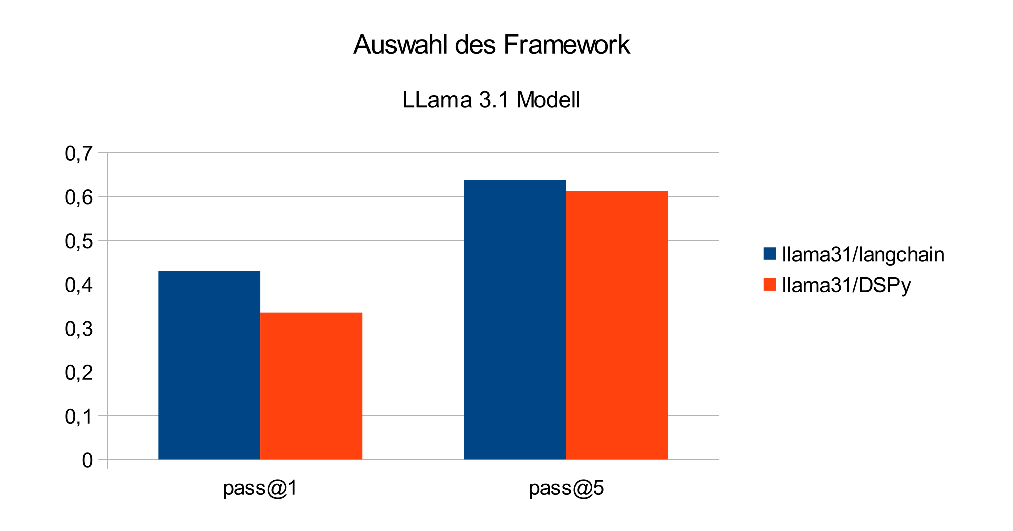
\includegraphics[width=0.5\textwidth]{content/chapter_evaluation/images/framework_evaluation_llama31.eps}\vspace{1cm}

	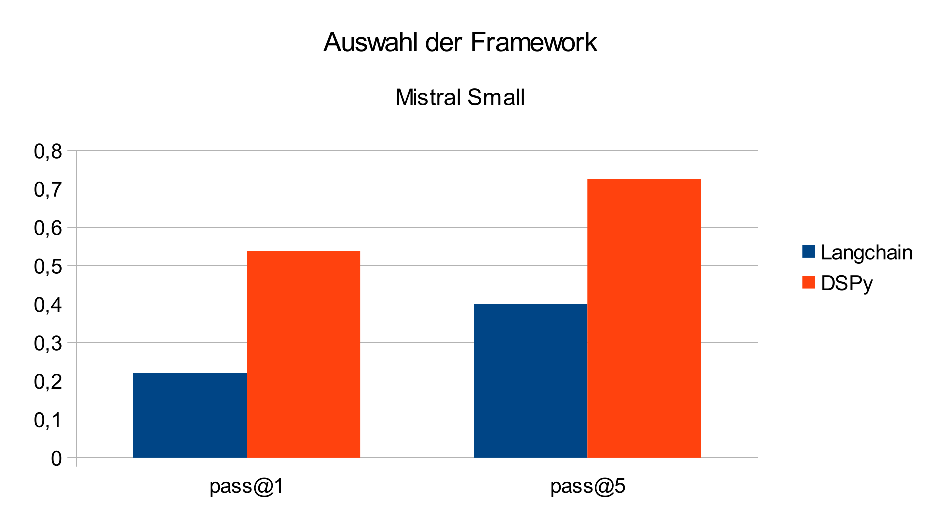
\includegraphics[width=0.5\textwidth]{content/chapter_evaluation/images/framework_evaluation_mistral-small.eps}
	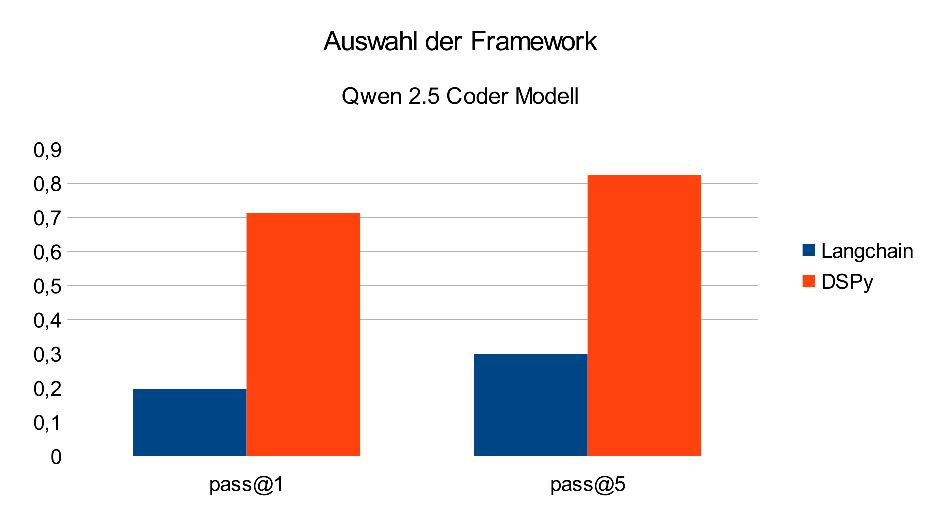
\includegraphics[width=0.5\textwidth]{content/chapter_evaluation/images/framework_evaluation_qwen25-coder.eps}
	\caption{Ergebnisse der pass@k-Methode für unterschiedliche Frameworks}
	\label{img:pass_at_k_results_by_framework}
\end{figure}

Die Werte aus der Abbildung \ref{img:pass_at_k_results_by_framework} sind in der Tabelle \ref{tab:pass_at_k_results_by_framework} detailliert aufgeführt. Zusätzlich ist der Tabelle die Differenz angegeben, welche zwischen den Ergebnissen der Frameworks \texttt{langchain} und \texttt{DSPy} festgehalten wurden. Die Differenz wurde nach der Formel $DPSy - langchain = Diff$ berechnet. Somit zeigt eine negative Differenz an, dass das Framework \texttt{langchain} bessere Werte erzielte, während eine positive Differenz anzeigt, dass das \texttt{DSPy}-Framework die besseren Ergebnisse erzielt hat.

\begin{table}[!ht]
	\begin{tabular}{|l|ll|ll|ll|ll|}
		\hline
		& \multicolumn{2}{c|}{\textbf{Codellama}} & \multicolumn{2}{c|}{\textbf{Llama3.1}} & \multicolumn{2}{c|}{\textbf{Qwen 2.5 Coder}} & \multicolumn{2}{c|}{\textbf{Mistral Small}} \\
		%\hline
		\textbf{k} & \textbf{1} & \textbf{5} & \textbf{1} & \textbf{5} & \textbf{1} & \textbf{5} & \textbf{1} & \textbf{5} \\
		\hline
		\textbf{Langchain}  & 0,005  & 0,025 & 0,43   & 0,6375 & 0,1975 & 0,3   & 0,22   & 0,4 \\
		\textbf{DSPy}       & 0,1425 & 0,4   & 0,335  & 0,6125 & 0,7125 & 0,825 & 0,5375 & 0,725 \\
		\hline
		\textbf{Diff}       & 0,1375 & 0,375 & -0,095 & -0,025 & 0,515  & 0,525 & 0,3175 & 0,325 \\
		\hline
		\hline
	\end{tabular}
	\centering
	\label{tab:pass_at_k_results_by_framework}
	\caption{Ergebnisse der pass@1 und pass@5 Methode verschiedener Frameworks}
\end{table}

Dieser Test zeigt, dass die Wahl des Famework für die Interaktion mit den Modellen, durchaus eine Verbesserung der Ergebnisse bewirken kann und durchaus in Erwägung gezogen werden sollte.
